\caulc
\begin{ex}%[1D6N3-2]%TDMZZ13- Nguyễn Sơn Thành-Trần Văn Thiện
	Tập xác định của hàm số $y=(x-1)^{-2}$ là
	\choice
	{$\mathbb{R}$}
	{\True $\mathbb{R} \setminus \{1\}$}
	{$\mathbb{R} \setminus \{0\}$}
	{$(0;+\infty)$}
	\loigiai{
		Hàm số $y=(x-1)^{-2}$ là hàm số lũy thừa có số mũ $\alpha = -2$ là một số nguyên âm.
		Do đó, hàm số xác định khi và chỉ khi $x-1 \neq 0 \Leftrightarrow x \neq 1$.\\
		Vậy tập xác định của hàm số là $\mathscr{D} = \mathbb{R} \setminus \{1\}$.
	}
\end{ex}

\begin{ex}%[1H8N7-1]%TDMZZ13- Nguyễn Sơn Thành-Trần Văn Thiện
	Thể tích của hình chóp có diện tích đáy bằng $B$ và chiều cao bằng $h$ tương ứng bằng
	\choice
	{$V = Bh$}
	{\True $V = \dfrac{1}{3}Bh$}
	{$V = \dfrac{1}{6}Bh$}
	{$V = \dfrac{\pi}{3}B^2h$}
	\loigiai{
		Thể tích của khối chóp có diện tích đáy $B$ và chiều cao $h$ được tính theo công thức $V = \dfrac{1}{3}Bh$.
	}
\end{ex}

\begin{ex}%[1D6H4-3]%TDMZZ13- Nguyễn Sơn Thành-Trần Văn Thiện
	Tập nghiệm của bất phương trình $\log\left(x^2 - 2x\right) < \log x$ là
	\choice
	{$\left(0;3\right)$}
	{$\left(\dfrac{7}{3};3\right)$}
	{$\left(3;+\infty\right)$}
	{\True $\left(2;3\right)$}
	\loigiai{
		Điều kiện xác định $\heva{&x^2-2x>0\\&x>0} \Leftrightarrow \heva{&\hoac{&x>2\\&x<0}\\&x>0} \Leftrightarrow x>2$.\\
		Với điều kiện trên, bất phương trình đã cho tương đương với
		$$x^2-2x<x\Leftrightarrow x^2-3x<0 \Leftrightarrow 0<x<3.$$
		Kết hợp với điều kiện $x>2$, ta được nghiệm của bất phương trình là $2<x<3$.\\
		Vậy tập nghiệm của bất phương trình là $S=\left(2;3\right)$.
	}
\end{ex}

\begin{ex}%[1H8V6-2]%TDMZZ13- Nguyễn Sơn Thành-Trần Văn Thiện
	\immini[thm]{
		Cho hình chóp đều $S. ABCD$ có tâm của đáy là $O$. Gọi $\varphi_1$, $\varphi_2$, $\varphi_3$ lần lượt là góc tạo bởi cạnh bên với đáy, cạnh bên với cạnh đáy, mặt bên với mặt đáy. Sắp xếp đúng theo chiều giảm dần là
		\choice
		{$\varphi_1$, $\varphi_2$, $\varphi_3$}
		{$\varphi_3$, $\varphi_1$, $\varphi_2$}
		{\True $\varphi_2$, $\varphi_3$, $\varphi_1$}
		{$\varphi_2$, $\varphi_1$, $\varphi_3$}
	}{
		\begin{tikzpicture}[scale=0.8, font=\footnotesize, line join=round, line cap=round, >=stealth]
			\coordinate (B) at (0,0);
			\coordinate (C) at (4,0);
			\coordinate (A) at (1.5,1.5);
			\coordinate (D) at (5.5,1.5);
			\coordinate (O) at ($(A)!0.5!(C)$);
			\coordinate (S) at ($(O)+(0,3.5)$);
			
			\draw[dashed] (B) -- (A) -- (D) (A) -- (C) (B) -- (D) (S) -- (A) (S) -- (O);
			\draw (S) -- (B) -- (C) -- (D) -- cycle (S) -- (C);
			
			\fill (S) circle (1.5pt) node[above] {$S$};
			\fill (A) circle (1.5pt) node[above right] {$A$};
			\fill (B) circle (1.5pt) node[left] {$B$};
			\fill (C) circle (1.5pt) node[below] {$C$};
			\fill (D) circle (1.5pt) node[right] {$D$};
			\fill (O) circle (1.5pt) node[below] {$O$};
		\end{tikzpicture}
	}
	\loigiai{
		\immini{
			Gọi $M$ là trung điểm của cạnh $CD$. Giả sử hình chóp tứ giác đều có cạnh đáy bằng $a$.\\
			Vì $S. ABCD$ là hình chóp đều nên hình chiếu của $S$ lên mặt đáy $(ABCD)$ chính là tâm $O$. Mặt khác, tam giác $SCD$ cân tại $S$ nên trung tuyến $SM$ đồng thời là đường cao, hay $SM \perp CD$.
			
		}{
			\begin{tikzpicture}[scale=0.8, font=\footnotesize, line join=round, line cap=round, >=stealth]
				\coordinate (B) at (0,0);
				\coordinate (C) at (4,0);
				\coordinate (A) at (1.5,1.5);
				\coordinate (D) at (5.5,1.5);
				\coordinate (O) at ($(A)!0.5!(C)$);
				\coordinate (S) at ($(O)+(0,3.5)$);
				\coordinate (M) at ($(C)!0.5!(D)$);
				
				\draw[dashed] (B) -- (A) -- (D) (A) -- (C) (B) -- (D) (S) -- (A) (S) -- (O) (O) -- (M);
				\draw (S) -- (B) -- (C) -- (D) -- cycle (S) -- (C) (S) -- (M);
				
				\fill (S) circle (1.5pt) node[above] {$S$};
				\fill (A) circle (1.5pt) node[above right] {$A$};
				\fill (B) circle (1.5pt) node[left] {$B$};
				\fill (C) circle (1.5pt) node[below] {$C$};
				\fill (D) circle (1.5pt) node[right] {$D$};
				\fill (O) circle (1.5pt) node[below left] {$O$};
				\fill (M) circle (1.5pt) node[right] {$M$};
			\end{tikzpicture}
		}
		\begin{itemize}
			\item Góc tạo bởi cạnh bên $SC$ và mặt đáy $(ABCD)$ là $\widehat{SCO}$, suy ra $\varphi_1 = \widehat{SCO}$.
			\item Góc tạo bởi cạnh bên $SC$ và cạnh đáy $CD$ là $\widehat{SCD}$, suy ra $\varphi_2 = \widehat{SCD}$.
			\item Góc tạo bởi mặt bên $(SCD)$ và mặt đáy $(ABCD)$ là $\widehat{SMO}$, suy ra $\varphi_3 = \widehat{SMO}$.
		\end{itemize}
		Xét tam giác $SOC$ vuông tại $O$, ta có $\tan \varphi_1 = \dfrac{SO}{OC}$.\\
		Xét tam giác $SOM$ vuông tại $O$, ta có $\tan \varphi_3 = \dfrac{SO}{OM}$.\\
		Vì $OC$ là nửa đường chéo và $OM$ là nửa cạnh của hình vuông $ABCD$ nên $OC > OM$.\\
		Do đó $\dfrac{SO}{OC} < \dfrac{SO}{OM} \Leftrightarrow \tan \varphi_1 < \tan \varphi_3 \Rightarrow \varphi_1 < \varphi_3$. \hfill (1)\\
		\noindent Lại có $OM = CM = \dfrac{a}{2}$. Xét $\cos \varphi_3 = \dfrac{OM}{SM}$ và $\cos \varphi_2 = \dfrac{CM}{SC}$.\\
		Trong tam giác vuông $SMC$ tại $M$, ta có $SM < SC$ (cạnh góc vuông luôn nhỏ hơn cạnh huyền).\\
		Suy ra $\dfrac{OM}{SM} > \dfrac{CM}{SC} \Leftrightarrow \cos \varphi_3 > \cos \varphi_2 \Rightarrow \varphi_3 < \varphi_2$. \hfill (2)\\
		Từ (1) và (2) suy ra $\varphi_2 > \varphi_3 > \varphi_1$.\\
		Sắp xếp theo chiều giảm dần ta được $\varphi_2, \varphi_3, \varphi_1$.
	}
\end{ex}

\begin{ex}%[2D1N1-2]%TDMZZ13- Nguyễn Sơn Thành-Trần Văn Thiện
	\immini[thm]{
		Cho hàm số $y=f(x)$ có đồ thị như hình vẽ bên. Hỏi hàm số $f(x)$ đồng biến trên khoảng nào dưới đây?
		\choice
		{$\left(-\infty;-2\right)$}
		{\True $\left(-2;1\right)$}
		{$\left(1;4\right)$}
		{$\left(1;+\infty\right)$}
	}{
		\begin{tikzpicture}[scale=0.6, font=\footnotesize,line join=round, line cap=round, >=stealth]		
			\draw[->] (-4.5,0)--(6.5,0) node[right]{$x$};
			\draw[->] (0,-4.2)--(0,4.5) node[above]{$y$};		
			\draw[blue,thick]
			(-3.8,3.1)--(-1.6,-3);		
			\draw[blue,thick,smooth,samples=200,domain=-1.6:6]
			plot(\x,{0.16*(\x-4)^2*(\x+1)});		
			\draw[dashed] (-1.6,0)--(-1.6,-3);
			\draw[dashed] (0.7,0)--(0.7,3);		
			\fill[blue] (-1.6,-3) circle(1.8pt);		
			\node[below left] at (0,0) {$O$};			
			\node[below] at (0.7,0) {$1$};
			\node[below] at (4,0) {$4$};			
			\node[above] at (-1.8,0) {$-2$};			
			\node[blue] at (5.2,3.5) {$f(x)$};			
		\end{tikzpicture}
	}
	\loigiai{
		Quan sát đồ thị hàm số $y=f(x)$, ta thấy đồ thị đi lên (từ trái sang phải) trên các khoảng $\left(-2;1\right)$ và $\left(4;+\infty\right)$.\\
		Do đó, hàm số đồng biến trên các khoảng $\left(-2;1\right)$ và $\left(4;+\infty\right)$.\\
		Đối chiếu với các đáp án, ta thấy khoảng $\left(-2;1\right)$ thỏa mãn yêu cầu bài toán.
	}
\end{ex}

\begin{ex}%[2H5N1-2]%TDMZZ13- Nguyễn Sơn Thành-Trần Văn Thiện
	Trong không gian hệ trục tọa độ $Oxyz$, cho mặt phẳng $(P)\colon 2x - y + z - 1 = 0$. Một vectơ pháp tuyến của mặt phẳng $(P)$ có tọa độ là
	\choice
	{\True $(2;-1;1)$}
	{$(2;1;1)$}
	{$(2;0;0)$}
	{$(2;1;-1)$}
	\loigiai{
		Mặt phẳng $(P)\colon 2x - y + z - 1 = 0$ có một vectơ pháp tuyến là $\overrightarrow{n} = (2;-1;1)$.
	}
\end{ex}

\begin{ex}%[2D1H4-1]%TDMZZ13- Nguyễn Sơn Thành-Trần Văn Thiện
	Cho hàm số $y=f(x)$ có bảng biến thiên như hình vẽ bên dưới. Đồ thị hàm số $y=f(x)$ có tất cả bao nhiêu đường tiệm cận (nếu chỉ xét tiệm cận đứng và tiệm cận ngang)?
	\begin{center}
		
\begin{tikzpicture}
			\tkzTabInit[nocadre=false,lgt=1.2,espcl=2.5,deltacl=0.6]
			{$x$ / 0.6, $f(x)$ / 2}
			{$-\infty$, $0$, $2$, $+\infty$}
			\tkzTabVar{+/ $+\infty$, -D-/ $3$ / $-\infty$, +D+/ $1$ / $+\infty$, -/ $0$}
		\end{tikzpicture}
	\end{center}
	\choice
	{\True $3$}
	{$4$}
	{$2$}
	{$1$}
	\loigiai{
		Dựa vào bảng biến thiên của hàm số $y=f(x)$, ta có
		\begin{itemize}
			\item $\lim\limits_{x \to 0^+} f(x) = -\infty$, suy ra đường thẳng $x=0$ là tiệm cận đứng của đồ thị hàm số.
			\item $\lim\limits_{x \to 2^+} f(x) = +\infty$, suy ra đường thẳng $x=2$ là tiệm cận đứng của đồ thị hàm số.
			\item $\lim\limits_{x \to +\infty} f(x) = 0$, suy ra đường thẳng $y=0$ là tiệm cận ngang của đồ thị hàm số.
			\item $\lim\limits_{x \to -\infty} f(x) = +\infty$, suy ra đồ thị hàm số không có tiệm cận ngang về phía $-\infty$.
		\end{itemize}
		Vậy đồ thị hàm số $y=f(x)$ có tất cả $3$ đường tiệm cận.
	}
\end{ex}

\begin{ex}%[2D4H1-3]%TDMZZ13- Nguyễn Sơn Thành-Trần Văn Thiện
	Họ nguyên hàm của hàm số $f(x)=2x-\cos x$ tương ứng là
	\choice
	{$x^2+\sin x+C$}
	{$2x^2+\sin x+C$}
	{$2x^2-\sin x+C$}
	{\True $x^2-\sin x+C$}
	\loigiai{
		Ta có $\displaystyle\int f(x)\mathrm{d}x = \displaystyle\int \left(2x - \cos x\right)\mathrm{d}x = x^2 - \sin x + C$.
	}
\end{ex}

\begin{ex}%[1D5H1-3]%TDMZZ13- Nguyễn Sơn Thành-Trần Văn Thiện
	Cho hai mẫu số liệu ghép nhóm $M_1$, $M_2$ với bảng tần số ghép nhóm:
	\begin{center}
		$M_1$ \quad
		\begin{tabular}{|c|c|c|c|c|c|c|}
			\hline
			Nhóm & $[2;3)$ & $[3;4)$ & $[4;5)$ & $[5;6)$ & $[6;7)$ & $[7;8)$ \\
			\hline
			Tần số & $3$ & $5$ & $6$ & $4$ & $6$ & $5$ \\
			\hline
		\end{tabular}
		\vspace{0.3cm}\\
		$M_2$ \quad
		\begin{tabular}{|c|c|c|c|c|c|c|}
			\hline
			Nhóm & $[4;6)$ & $[6;8)$ & $[8;10)$ & $[10;12)$ & $[12;14)$ & $[14;16)$ \\
			\hline
			Tần số & $3$ & $5$ & $6$ & $4$ & $6$ & $5$ \\
			\hline
		\end{tabular}
	\end{center}
	Hãy so sánh số trung bình cộng $\overline{x}_1$, $\overline{x}_2$ của hai mẫu số liệu $M_1$, $M_2$?
	\choice
	{$\overline{x}_1 = \overline{x}_2$}
	{$\overline{x}_1 < \overline{x}_2$}
	{$\overline{x}_1 > \overline{x}_2$}
	{\True $\overline{x}_2 = 2\overline{x}_1$}
	\loigiai{
		Số phần tử của hai mẫu số liệu đều là $n = 3 + 5 + 6 + 4 + 6 + 5 = 29$.\\
		Đối với mẫu số liệu $M_1$, các giá trị đại diện lần lượt là: $2{,}5$; $3{,}5$; $4{,}5$; $5{,}5$; $6{,}5$; $7{,}5$.\\
		Số trung bình cộng của mẫu $M_1$ là
		$$ \overline{x}_1 = \frac{2{,}5 \cdot 3 + 3{,}5 \cdot 5 + 4{,}5 \cdot 6 + 5{,}5 \cdot 4 + 6{,}5 \cdot 6 + 7{,}5 \cdot 5}{29} = \frac{150{,}5}{29}. $$
		Đối với mẫu số liệu $M_2$, các giá trị đại diện lần lượt là: $5$; $7$; $9$; $11$; $13$; $15$.\\
		Số trung bình cộng của mẫu $M_2$ là
		$$ \overline{x}_2 = \frac{5 \cdot 3 + 7 \cdot 5 + 9 \cdot 6 + 11 \cdot 4 + 13 \cdot 6 + 15 \cdot 5}{29} = \dfrac{301}{29}. $$
		Ta thấy $\dfrac{301}{29} = 2 \cdot \dfrac{150{,}5}{29}$, suy ra $\overline{x}_2 = 2\overline{x}_1$.\\
		\textit{Cách giải nhanh:} Nhận thấy các tần số tương ứng của hai mẫu số liệu là bằng nhau và giá trị đại diện mỗi nhóm của mẫu $M_2$ đều gấp $2$ lần giá trị đại diện nhóm tương ứng của mẫu $M_1$ nên ta suy ra ngay $\overline{x}_2 = 2\overline{x}_1$.
	}
\end{ex}

\begin{ex}%[2D4V3-1]%TDMZZ13- Nguyễn Sơn Thành-Trần Văn Thiện
	\immini[thm]{
		Cho hình phẳng $(H)$ giới hạn bởi các đường cong $y=f(x)$, $y=g(x)$ và trục hoành như hình vẽ. Công thức tính diện tích hình phẳng $(H)$ là
	}{
		\begin{tikzpicture}[>=stealth, scale=0.8, line join=round, line cap=round]
			\draw[->] (-1,0) -- (6,0) node[below] {$x$};
			\draw[->] (0,-1) -- (0,4) node[right] {$y$};
			\node[below right] at (0,0) {$O$};
			\draw (2,0) node[below] {$2$};
			\draw (5,0) node[below] {$5$};
			\draw[dashed] (5,0) -- (5,3.2);			
			% Tô màu vùng (H)
			\path[pattern=north east lines, pattern color=gray] 
			(0,0) .. controls (0.5,1.5) and (2.5,2.5) .. (5,3.2) -- (2,0) -- cycle;			
			% Vẽ đồ thị f(x)
			\draw[blue, thick] (0,0) .. controls (0.5,1.5) and (2.5,2.5) .. (5.5,3.4) ;
			\node at (3,2.5)[above] {$f(x)$};
			% Vẽ đồ thị g(x)
			\draw[blue, thick] (1,-1.06) -- (5.5,3.73);
			\node at (3.2,1)[below] {$g(x)$};
			\node at (2.2,1.2) {$(H)$};
		\end{tikzpicture}
	}
	\choice
	{$\displaystyle\int\limits_0^2 f(x)\mathrm{\,d}x + \displaystyle\int\limits_2^5 g(x)\mathrm{\,d}x$}
	{$\displaystyle\int\limits_0^2 \left[g(x) - f(x)\right]\mathrm{\,d}x + \displaystyle\int\limits_2^5 \left[f(x) - g(x)\right]\mathrm{\,d}x$}
	{\True $\displaystyle\int\limits_0^2 f(x)\mathrm{\,d}x + \displaystyle\int\limits_2^5 \left[f(x) - g(x)\right]\mathrm{\,d}x$}
	{$\displaystyle\int\limits_0^2 g(x)\mathrm{\,d}x + \displaystyle\int\limits_2^5 \left[g(x) - f(x)\right]\mathrm{\,d}x$}
	\loigiai{
		Dựa vào hình vẽ, ta thấy diện tích hình phẳng $(H)$ được chia làm hai phần:
		\begin{itemize}
			\item Phần thứ nhất ứng với $x \in [0;2]$: Hình phẳng giới hạn bởi đồ thị $y=f(x)$, trục hoành $y=0$, đường thẳng $x=0$ và $x=2$. Nhận thấy trên đoạn này $f(x) \ge 0$, nên diện tích phần này là $S_1 = \displaystyle\int\limits_0^2 f(x)\mathrm{\,d}x$.
			\item Phần thứ hai ứng với $x \in [2;5]$: Hình phẳng giới hạn bởi đồ thị $y=f(x)$, đường thẳng $y=g(x)$, đường thẳng $x=2$ và $x=5$. Nhận thấy trên đoạn này đồ thị $y=f(x)$ nằm phía trên đường thẳng $y=g(x)$, nên diện tích phần này là $S_2 = \displaystyle\int\limits_2^5 \left[f(x) - g(x)\right]\mathrm{\,d}x$.
		\end{itemize}
		Vậy công thức tính diện tích hình phẳng $(H)$ là
		$$S = S_1 + S_2 = \displaystyle\int\limits_0^2 f(x)\mathrm{\,d}x + \displaystyle\int\limits_2^5 \left[f(x) - g(x)\right]\mathrm{\,d}x.$$
	}
\end{ex}

\begin{ex}%[2H2H2-4]%TDMZZ13- Nguyễn Sơn Thành-Trần Văn Thiện
	Trong không gian $Oxyz$, cho hai véc-tơ $\overrightarrow{u} = (3;-1;-2)$ và $\overrightarrow{v} = (-1;-2;0)$. Tích vô hướng $\overrightarrow{u} \cdot \overrightarrow{v}$ bằng
	\choice
	{$1$}
	{\True $-1$}
	{$2$}
	{$-2$}
	\loigiai{
		Ta có $\overrightarrow{u} \cdot \overrightarrow{v} = 3 \cdot (-1) + (-1) \cdot (-2) + (-2) \cdot 0 = -3 + 2 + 0 = -1$.
	}
\end{ex}

\begin{ex}%[2H2H1-1]%TDMZZ13- Nguyễn Sơn Thành-Trần Văn Thiện
	Trong không gian cho hình bình hành $ABCD$, với một điểm $M$ bất kì luôn có $\overrightarrow{MA} + \overrightarrow{MB} + \overrightarrow{MC} + \overrightarrow{MD} = 4\overrightarrow{MO}$. Điểm $O$ là
	\choice
	{\True trung điểm của $AC$}
	{trung điểm của $AB$}
	{trung điểm của $AD$}
	{trung điểm của $BC$}
	\loigiai{
		Gọi $O'$ là tâm của hình bình hành $ABCD$. Do đó, $O'$ lần lượt là trung điểm của $AC$ và $BD$.\\
		Với một điểm $M$ bất kì trong không gian, ta luôn có
		\begin{eqnarray*}
			\overrightarrow{MA} + \overrightarrow{MC} &=& 2\overrightarrow{MO'}\\
			\overrightarrow{MB} + \overrightarrow{MD} &=& 2\overrightarrow{MO'}
		\end{eqnarray*}
		Cộng vế với vế hai đẳng thức trên ta được
		$$\overrightarrow{MA} + \overrightarrow{MB} + \overrightarrow{MC} + \overrightarrow{MD} = 4\overrightarrow{MO'}.$$
		Mà theo giả thiết ta có $\overrightarrow{MA} + \overrightarrow{MB} + \overrightarrow{MC} + \overrightarrow{MD} = 4\overrightarrow{MO}$.\\
		Từ đó suy ra $4\overrightarrow{MO'} = 4\overrightarrow{MO} \Leftrightarrow \overrightarrow{MO'} = \overrightarrow{MO} \Leftrightarrow O \equiv O'$.	\\
		Vậy $O$ là trung điểm của $AC$.
	}
\end{ex}
\cauds
\begin{ex}%[2D1V5-8]%[Dương Công Tạo]
	Doanh thu khi bán một loại sản phẩm X được mô hình hoá bởi hàm $S(t) = \dfrac{at + b}{t + d}$ (số sản phẩm bán được sau $t$ ngày), với ($t \ge 0$). Biết số lượng sản phẩm bán được sau một ngày là $112$ sản phẩm, bán được trong ngày thứ hai là $56$ sản phẩm.
	\choiceTF
	{$a+d=336$}
	{\True Trong ngày thứ $7$ bán được $9$ sản phẩm (làm tròn tới hàng đơn vị)}
	{\True Số lượng sản phẩm X bán được sẽ không vượt quá $336$ sản phẩm}
	{Để đảm bảo cho tính tối ưu khi mà tính toán theo lí thuyết số lượng sản phẩm X bán được trong một ngày nhỏ hơn $3$ sản phẩm thì sẽ dùng lại không bán sản phẩm X nữa. Việc bán sản phẩm X sẽ dừng lại sau $12$ ngày bán}
	\loigiai{
		Theo giả thiết, ta có
		\begin{itemize}
			\item $S(0)=0 \Rightarrow \dfrac{b}{d}=0 \Rightarrow b=0$; $S(t) = \dfrac{at}{t+d}$.
			\item $S(1)=112 \Rightarrow \dfrac{a}{1+d}=112\Leftrightarrow a=112(1+d)$.\quad(1)
			\item $S(2)-S(1)=56 \Rightarrow S(2)=S(1)+56=112+56=168$.\\
			Khi đó $S(2)=168\Leftrightarrow \dfrac{2a}{2+d}=168 \Rightarrow a=84(2+d)$.\quad(2)\\
			Từ (1) và (2) ta có $112(1+d)=84(2+d) \Rightarrow 112+112d=168+84d \Rightarrow 28d=56 \Rightarrow d=2$. \\
			Khi đó $a=112(1+2)=336$.
		\end{itemize}
		Vậy $a=336$, $d=2$ và $S(t)=\dfrac{336t}{t+2}$.
		\begin{itemchoice}
			\itemch $a+d=336+2=338$.
			\itemch $S(7)-S(6)=\dfrac{336\cdot 7}{7+2} - \dfrac{336\cdot 6}{6+2} = \dfrac{336\cdot 7}{9} - \dfrac{336\cdot 6}{8} =\dfrac{28}{3}\approx 9$ (sản phẩm).
			\itemch $\lim\limits_{t \to \infty} S(t) = \lim\limits_{t \to \infty} \dfrac{336t}{t+2} = 336$. \\
			Vậy số lượng sản phẩm X bán được sẽ không vượt quá $336$ sản phẩm.
			\itemch Ta có \allowdisplaybreaks
			\begin{eqnarray*}
				S(t)-S(t-1)&=& \dfrac{336t}{t+2} - \dfrac{336(t-1)}{t+1} \\
				&=& 336\cdot \left[\dfrac{t(t+1)-(t-1)(t+2)}{(t+1)(t+2)}\right] \\
				&=& 336\cdot \dfrac{t^2+t-(t^2+t-2)}{(t+1)(t+2)} \\
				&=& \dfrac{672}{(t+1)(t+2)}.
			\end{eqnarray*}
			Để $S(t)-S(t-1) < 3$ thì \allowdisplaybreaks
			\begin{eqnarray*}
				&&\dfrac{672}{(t+1)(t+2)} < 3 \\
				&\Leftrightarrow&(t+1)(t+2) > \dfrac{672}{3}\\
				&\Leftrightarrow&t^2+3t+2 > 224 \\
				&\Leftrightarrow&t^2+3t-222 > 0\\
				&\Leftrightarrow&t<\dfrac{-3-\sqrt{897}}{2}\text{ hoặc }t>\dfrac{-3+\sqrt{897}}{2}.
			\end{eqnarray*}
			Vì $t\geq 0$ nên $t>\dfrac{-3+\sqrt{897}}{2}\approx 13{,}475$.\\
			Vậy $t$ nguyên nhỏ nhất là $14$.
		\end{itemchoice}
	}
\end{ex}

\begin{ex} %[TDMZZ13-14-DS]%[Hà Văn Hảo]%[2D4H2-1]
	Cho hai hàm số $f(x)$ và $g(x)$ có đạo hàm xác định trên $\mathbb{R}$ và thoả mãn $\displaystyle\int x f(x)\,\mathrm{d}x = x^4 - 4x^3 + C$, $\displaystyle\int g(x)\,\mathrm{d}x = f'(x) + C$.
	\choiceTF
	{$f(x) = 4x^3 - 12x^2$}
	{$g(x) = 8x - 12$}
	{\True $\displaystyle\int\limits_0^1 [f(x) + g(x)]\,\mathrm{d}x = \displaystyle\int\limits_0^1 f(x)\,\mathrm{d}x + \displaystyle\int\limits_0^1 g(x)\,\mathrm{d}x$}
	{\True $\displaystyle\int\limits_0^1 f(x)g(x)\,\mathrm{d}x = \displaystyle\int\limits_0^1 f(x)\,\mathrm{d}x \cdot \displaystyle\int\limits_0^1 g(x)\,\mathrm{d}x$}
	\loigiai{
		\begin{itemchoice}
			\itemch Ta có $\left(\displaystyle\int x f(x)\,\mathrm{d}x\right)' = (x^4 - 4x^3 + C)' \Leftrightarrow x f(x) = 4x^3 - 12x^2 \Rightarrow f(x) = 4x^2 - 12x$.
			\itemch Từ $f(x) = 4x^2 - 12x \Rightarrow f'(x) = 8x - 12$.\\
			Theo giả thiết $\displaystyle\int g(x)\,\mathrm{d}x = 8x - 12 + C$.\\
			Suy ra $\left(\displaystyle\int g(x)\,\mathrm{d}x\right)' = (8x - 12 + C)' = 8$.
			\itemch Dựa vào tính chất của tích phân $\displaystyle\int\limits_a^b [f(x) \pm g(x)]\,\mathrm{d}x = \displaystyle\int\limits_a^b f(x)\,\mathrm{d}x \pm \displaystyle\int\limits_a^b g(x)\,\mathrm{d}x$.
			\itemch Tích phân của một tích không bằng tích các tích phân, nhưng $g(x)=8$ và $\displaystyle\int\limits_0^1 g(x)\,\mathrm{d}x=8$.\\
			Vậy $\displaystyle\int\limits_0^1 [f(x) \cdot g(x)]\,\mathrm{d}x = \displaystyle\int\limits_0^1 f(x)\,\mathrm{d}x \cdot \displaystyle\int\limits_0^1 g(x)\,\mathrm{d}x$.
		\end{itemchoice}
	}
\end{ex}

\begin{ex}%[2D6C2-4]%[TDMZZ13]%[Vũ Hồng Toàn]
	Theo thống kê hiện tại có một dịch bệnh X rất nguy hiểm và đang có $4\%$ dân số thật sự mắc bệnh này. Một công ty có đề xuất một loại dụng cụ TEST X cho khả năng phát hiện chuẩn đến $90\%$ một loại bệnh X. Tuy nhiên, TEST X cũng cho kết quả \lq\lq dương tính giả\rq\rq cho một người không bị bệnh X tới $6\%$ (tức là một người không bị bệnh X mà dùng TEST X sẽ cho kết quả dương tính là $6\%$). Chọn ngẫu nhiên một người dân và cho sử dụng hệ thống TEST X. Gọi $A$ là biến cố người dân được chọn bị nhiễm bệnh X thật sự, $B$ là biến cố người dân này bị dụng cụ TEST báo dương tính.
	\choiceTF
	{\True $\mathrm{P}(A)=0{,}04$}
	{\True $\mathrm{P}\left(\overline{B} \mid \overline{A}\right)=0{,}94$}
	{\True Xác suất để hệ thống TEST báo kết quả dương tính là $\dfrac{117}{1\,250}$}
	{\True $\mathrm{P}\left(A \mid \overline{B}\right)=\dfrac{5}{1\,133}$}
	\loigiai{
		Từ giả thiết của bài toán, ta có các thông tin sau:
		\begin{itemize}
			\item $\mathrm{P}(A) = 4\% = 0{,}04 \Rightarrow \mathrm{P}\left(\overline{A}\right) = 1 - 0{,}04 = 0{,}96$.
			\item Khả năng phát hiện chuẩn đến $90\%$ nên $\mathrm{P}(B \mid A) = 90\% = 0{,}9 \Rightarrow \mathrm{P}\left(\overline{B} \mid A\right) = 1 - 0{,}9 = 0{,}1$.
			\item Tỉ lệ \lq\lq dương tính giả\rq\rq là $6\%$ nên $\mathrm{P}\left(B \mid \overline{A}\right) = 6\% = 0{,}06 \Rightarrow \mathrm{P}\left(\overline{B} \mid \overline{A}\right) = 1 - 0{,}06 = 0{,}94$.
		\end{itemize}
		\begin{itemchoice}
			\itemch Vì theo giả thiết $\mathrm{P}(A) = 0{,}04$.
			\itemch Vì $\mathrm{P}(\overline{B} \mid \overline{A}) = 1 - \mathrm{P}(B \mid \overline{A}) = 1 - 0{,}06 = 0{,}94$.
			\itemch Xác suất để hệ thống TEST báo kết quả dương tính là
			\allowdisplaybreaks
			\begin{eqnarray*}
				\mathrm{P}(B) &=& \mathrm{P}(A) \cdot \mathrm{P}(B \mid A) + \mathrm{P}\left(\overline{A}\right) \cdot \mathrm{P}\left(B \mid \overline{A}\right)\\
				&=& 0{,}04 \cdot 0{,}9 + 0{,}96 \cdot 0{,}06 \\
				&=& \dfrac{117}{1\,250}.
			\end{eqnarray*}
			\itemch Xác suất để một người bị bệnh khi kết quả TEST âm tính là
			\[\mathrm{P}\left(A \mid \overline{B}\right) = \dfrac{\mathrm{P}\left(A \cap \overline{B}\right)}{\mathrm{P}\left(\overline{B}\right)} = \dfrac{\mathrm{P}(A) \cdot \mathrm{P}\left(\overline{B} \mid A\right)}{1 - \mathrm{P}(B)} = \dfrac{0{,}04 \cdot 0{,}1}{1 - 0{,}0936} = \dfrac{5}{1\,133}.\]
		\end{itemchoice}
	}
\end{ex}

\begin{ex}%[2H5C3-4]%[TDMZZ13]%[Văn Minh Thoại]
	\def\dotEX{}
	Trong không gian $Oxyz$ có đơn vị dài trên mỗi trục là centimet, cho một quả cầu đặc $(S)$ có bán kính bằng $22$ cm ban đầu có tâm đang ở điểm $A(190;0;0)$ và một bức tường đủ rộng nằm trên mặt phẳng $(\alpha)\colon x=0$. Quả cầu bắt đầu chuyển động thẳng về phía bức tường theo hướng của vectơ $\overrightarrow{u}=(-1;2;2)$ với tốc độ không đổi bằng $20$ cm/s.
	\choiceTF
	{\True $\mathrm{d}\big(A,(\alpha)\big)=190$.}
	{\True Tâm của quả cầu $(S)$ chuyển động trên đường thẳng $\heva{&x=190-t\\&y=2t\\&z=2t.}$}
	{Sau khi chuyển động được $5$ giây thì tâm quả cầu cách bức tường một khoảng bằng $65$ cm \textit{(tính theo centimet và làm tròn đến hàng đơn vị)}.}
	{Tính từ lúc bắt đầu chuyển động đến khi quả cầu va chạm vào bức tường thì hết một khoảng thời gian là $9{,}5$ giây \textit{(tính theo giây và làm tròn đến hàng phần mười)}.}
	\loigiai{
		\begin{itemchoice}
			\itemch Khoảng cách từ điểm $A(190;0;0)$ đến mặt phẳng $(\alpha)\colon x=0$ là
			\[\mathrm{d}\big(A, (\alpha)\big) = \dfrac{|190|}{\sqrt{1^2+0^2+0^2}} = 190\;\text{ (cm)}.\]
			\itemch Tâm quả cầu bắt đầu chuyển động từ điểm $A(190;0;0)$ theo hướng của vectơ $\overrightarrow{u}=(-1;2;2)$ có quỹ đạo chuyển động là đường thẳng
			$\heva{&x=190-t\\&y=2t\\&z=2t}\quad(t\in\mathbb{R})$.
			\itemch Tại thời điểm $t=5$ (s), với tốc độ $v=20$ cm/s, quãng đường tâm quả cầu di chuyển được là
			\[AB = v \cdot t = 20 \cdot 5 = 100\;\text{(cm)}.\]
			Gọi $B$ là vị trí tâm quả cầu sau $5$ giây. \\
			Ta có vectơ $\overrightarrow{AB}$ cùng hướng với $\overrightarrow{u}$ và độ dài $AB=100$.\\
			Mặt khác, $\left|\overrightarrow{u}\right|=\sqrt{(-1)^2+2^2+2^2}=3$. Suy ra
			\[\overrightarrow{AB} = \dfrac{AB}{\left|\overrightarrow{u}\right|} \overrightarrow{u} = \dfrac{100}{3} (-1;2;2) = \left(-\dfrac{100}{3}; \dfrac{200}{3}; \dfrac{200}{3}\right).\]
			Tọa độ điểm $B$ là $B=A+\overrightarrow{AB}=\left(\dfrac{470}{3};\dfrac{200}{3};\dfrac{200}{3}\right)$.\\
			Khoảng cách từ tâm $B$ đến bức tường $(\alpha)\colon x=0$ là
			\[\mathrm{d}\big(B, (\alpha)\big) = \left|x_B\right| = \dfrac{470}{3}\approx 157\;\text{(cm)}.\]
			\itemch
			\begin{center}
				\begin{tikzpicture}[declare function={r = 1.2;},line join=round,line cap=round,>=stealth,scale=1,font=\footnotesize]
					\fill[pattern = bricks, pattern color = brown] (-0.5,0) rectangle (0,6.5);
					\draw (0,0) -- (0,6.5) node[above] {$(\alpha)\colon x=0$};
					\path
					(7.5,5.5) coordinate (A)
					(0,5.5) coordinate (H)
					(r,1.5) coordinate (D)
					(0,1.5) coordinate (K)
					(r,5.5) coordinate (M);
					\draw (D) circle (r);
					\draw[dashed] (A) -- (M) node[pos=0.5,sloped,above] {$\Delta\mathrm{d}$};
					\draw[dashed] (M) -- (H) node[pos=0.5,sloped,above] {$22$};
					\draw[dashed] (D) -- (K) node[pos=0.5,sloped,below,font=\scriptsize] {$R=22$};
					\draw[dashed] (D) -- (M);
					\draw[->] (A) -- (D);
					\foreach \x/\y/\z in {A/D/M}{
						\path (\y) pic[draw,angle radius=8mm,angle eccentricity=0.5,"$\varphi$"]{angle = \x--\y--\z};
					} \draw[->] (0,3.5) -- (1.5,3.5) node[right] {$\overrightarrow{n}$};
					\foreach \p/\pos in {A/0,D/-50,M/90}{
						\draw[fill,ball color=red] (\p) circle (1pt) node[shift={(\pos:4mm)},font=\footnotesize] {$\p$};
					}
					\foreach \x/\y/\z in {K/H/M,D/M/A,D/K/H}{
						\path (\y) pic[draw,angle radius=5pt]{right angle = \x--\y--\z};
					}
				\end{tikzpicture}
			\end{center}
			Vectơ pháp tuyến của mặt phẳng $(\alpha)$ là $\overrightarrow{n}=(1;0;0)$.\\
			Gọi $\varphi$ là góc giữa đường thẳng quỹ đạo (có VTCP $\overrightarrow{u}$) và mặt phẳng $(\alpha)$. Ta có
			\[\sin \varphi = \left|\cos\left(\overrightarrow{u}, \overrightarrow{n}\right)\right| = \dfrac{\left|\overrightarrow{u} \cdot \overrightarrow{n}\right|}{\left|\overrightarrow{u}\right| \cdot \left|\overrightarrow{n}\right|} = \dfrac{|-1 \cdot 1 + 2 \cdot 0 + 2 \cdot 0|}{3 \cdot 1} = \dfrac{1}{3}.\]
			Gọi $D$ là vị trí tâm quả cầu ngay tại thời điểm quả cầu vừa va chạm vào mặt tường.\\
			Lúc này, khoảng cách từ $D$ đến mặt phẳng $(\alpha)$ chính bằng bán kính quả cầu là
			\[\mathrm{d}\big(D, (\alpha)\big) = R = 22\;\text{(cm)}.\]
			Khoảng cách theo phương vuông góc với mặt phẳng $(\alpha)$ mà quả cầu đã tiến lại gần bức tường là
			\[\Delta \mathrm{d} = \mathrm{d}\big(A, (\alpha)\big) - \mathrm{d}\big(D, (\alpha)\big) = 190 - 22 = 168\;\text{(cm)}.\]
			Quãng đường thực tế $AD$ mà tâm quả cầu đã di chuyển trên quỹ đạo là
			\[AD = \dfrac{\Delta \mathrm{d}}{\sin \varphi} = \dfrac{168}{\dfrac{1}{3}} = 504\;\text{(cm)}.\]
			Thời gian chuyển động để quả cầu va chạm vào bức tường là
			\[t = \dfrac{AD}{v} = \dfrac{504}{20} = 25{,}2\;\text{(s)}.\]
		\end{itemchoice}
	}
\end{ex}
\caukq 

\begin{ex}%[1H8H6-2]%[TDMZZ13]%[Lê Hồ Quang Minh]
	Cho hình chóp $S.ABCD$ có đáy là hình vuông cạnh bằng $4$, cạnh bên $SA$ vuông góc với đáy và có $SA = 5$. Hãy xác định số đo góc nhị diện $[S, BD, C]$ theo đơn vị độ \textit{(làm tròn kết quả đến hàng đơn vị)}?
	\par
	\shortans[0]{119}
	\loigiai{
		\immini{Gọi $O$ là giao điểm của $AC$ và $BD$. Vì $ABCD$ là hình vuông nên $AC \perp BD$ tại $O$.\\
			Ta có $\heva{&BD \perp AO \\ &BD \perp SA \text{ (do } SA \perp (ABCD)\text{)}} \Rightarrow BD \perp (SAO) \Rightarrow BD \perp SO$.\\
			Do đó góc nhị diện $[S, BD, A]$ chính là góc phẳng nhị diện $\widehat{SOA}$.\\
			Xét tam giác $SAO$ vuông tại $A$, ta có
			\[ \tan\widehat{SOA} = \dfrac{SA}{AO} = \dfrac{5}{2\sqrt{2}}\]
			Vậy số đo góc nhị diện cần tìm là
			\[[S, BD, C] = 180^\circ - \arctan\left(\dfrac{5}{2\sqrt{2}}\right) \approx 119^\circ. \]}
		{\begin{tikzpicture}[scale=0.7, font=\footnotesize,line join=round, line cap=round, >=stealth]
				\path 
				(0,0) coordinate (A)
				++(-140:2) coordinate (B)
				++(0:3.5) coordinate (C)
				($(A)+(C)-(B)$) coordinate (D)
				($(A)+(0,3)$) coordinate (S)
				($(A)!0.5!(C)$) coordinate (O)
				;
				\foreach \i in{B,C,D}{\draw (S)--(\i);};
				\draw (B)--(C)--(D);
				\draw[dashed] (O)--(S)--(A)--(B) (C)--(A)--(D)--(B);
				\pic[draw,angle eccentricity=1.8,angle radius=2mm]{right angle=S--A--D};
				\foreach \i/\g in {A/-90,B/-90,C/-90,D/-90,S/90,O/-90}
				\fill[black] (\i) circle(1pt)+(\g:3mm)node[scale=1]{$\i$};
		\end{tikzpicture}}
	}
\end{ex}

\begin{ex}%[Duong Xuan Loi]%[2D4V2-6]
	Tốc độ thay đổi của số lượng vi khuẩn trong $1$ ml nước ở hồ bơi $X$ tại thời điểm $t$ (ngày), tính từ lúc hồ nước vừa được xử lí an toàn, được mô hình bởi hàm số
	\[
	f'(t)=\dfrac{1\,500}{(1+0{,}25t)^2}\quad (\text{con/ngày}),\ t\ge 0.
	\]
	Biết rằng số lượng vi khuẩn ban đầu là $300$ con trên mỗi ml nước và mức độ an toàn cho người sử dụng hồ bơi là số vi khuẩn phải ít hơn $3\,800$ con trên mỗi ml nước. Biết rằng sau tối đa $n$ ngày thì người ta phải xử lí và thay nước mới cho hồ bơi để đảm bảo an toàn cho người sử dụng. Hãy tính $n$.
	\par\shortans[oly]{5}
	\loigiai{
		Gọi $f(t)=\dfrac{at+b}{1+0{,}25t}$ là số lượng vi khuẩn trong $1$ ml nước tại thời điểm $t$.\\
		Theo giả thiết
		\[
		\heva{& f'(t)=\dfrac{1\,500}{(1+0{,}25t)^2} \\ & f(0)=300}\Leftrightarrow \heva{&a-0{,}25=1\,500 \\ & b=300}\Leftrightarrow \heva{& a=1\,575 \\ & b=300}
		\]
		Vậy $f(t)=\dfrac{1\,575t+300}{1+0{,}25t}$.\\
		Điều kiện an toàn:
		\[
		f(t)<3\,800\Leftrightarrow \dfrac{1\,575t+300}{1+0{,}25t}<3\,800
		\Leftrightarrow 1\,575t+300<3\,800+950t \Leftrightarrow t<5{,}6.
		\]
		Vậy sau tối đa $5$ ngày thì phải xử lí và thay nước mới.\\
		Do đó $n=5$.
	}
\end{ex}

\begin{ex}%[2D6C1-2]
	Cho hai hộp, ban đầu hộp I đựng $5$ viên bi đỏ và $4$ viên bi xanh, hộp II đựng $6$ viên bi đỏ và $2$ viên bi xanh, $1$ viên bi vàng. Tiến hành lấy ngẫu nhiên $2$ viên bi từ hộp I bỏ sang hộp II. Sau đó, tiến hành lấy ngẫu nhiên $2$ viên bi từ hộp II bỏ sang hộp I. Hãy tính xác suất để hộp I có đủ $3$ màu, nếu biết hộp II có số bi đỏ nhỏ hơn $6$ (\textit{làm tròn kết quả đến hàng phần trăm})?
	\begin{center}
		\begin{tikzpicture}[line join = round, line cap=round,>=stealth,font=\footnotesize,scale=1]
			% Hộp I
			\draw[thick] (0,0) rectangle (4,2.5);
			\node at (2,2.8) {\text{Hộp I}};
			\filldraw[red, draw=yellow] (0.5,0.5) circle (0.25);
			\filldraw[red, draw=yellow] (1.5,0.5) circle (0.25);
			\filldraw[red, draw=yellow] (2.5,0.5) circle (0.25);
			\filldraw[red, draw=yellow] (1,1.25) circle (0.25);
			\filldraw[red, draw=yellow] (2,2) circle (0.25);
			\filldraw[cyan, draw=yellow] (0.5,1.75) circle (0.25);
			\filldraw[cyan, draw=yellow] (1.5,1.75) circle (0.25);
			\filldraw[cyan, draw=yellow] (3.5,0.5) circle (0.25);
			\filldraw[cyan, draw=yellow] (3.5,1.75) circle (0.25);
			
			% Hộp II
			\draw[thick] (5,0) rectangle (9,2.5);
			\node at (7,2.8) {\text{Hộp II}};
			\filldraw[red, draw=yellow] (5.5,0.5) circle (0.25);
			\filldraw[red, draw=yellow] (6.5,1.25) circle (0.25);
			\filldraw[red, draw=yellow] (7.5,1.25) circle (0.25);
			\filldraw[red, draw=yellow] (8.5,1.75) circle (0.25);
			\filldraw[red, draw=yellow] (8.5,0.5) circle (0.25);
			\filldraw[red, draw=yellow] (6.5,2) circle (0.25);
			\filldraw[yellow, draw=yellow] (5.5,1.5) circle (0.25);
			\filldraw[cyan, draw=yellow] (6.5,0.5) circle (0.25);
			\filldraw[cyan, draw=yellow] (7.5,0.5) circle (0.25);
		\end{tikzpicture}
	\end{center}
	\par\shortans{0,05}
	\loigiai{
		Gọi $A$ là biến cố \lq\lq Hộp I có đủ 3 màu\rq\rq.\\
		Gọi $B$ là biến cố \lq\lq Hộp II có số bi đỏ nhỏ hơn 6\rq\rq.\\
		Ta cần tính $P(A\mid B) = \dfrac{n(A \cap B)}{P(A)}$.\\
		Ban đầu, hộp I có $5$ viên bi đỏ và $4$ viên bi xanh ($5$Đ, $4$X), hộp II có $6$ viên bi đỏ và $2$ viên bi xanh, $1$ viên bi vàng ($6$Đ, $2$X, $1$V). Lấy $2$ viên từ I sang II, ta có các trường hợp sau
		\begin{itemize}
			\item \textbf{TH1} Lấy $2$Đ từ hộp I sang hộp II. Khi đó hộp II có $8$Đ, $2$X, $1$V. Để hộp II có số bi đỏ nhỏ hơn $6$ thì ta phải lấy nhiều hơn $2$ viên bi đỏ từ hộp II, điều này không thỏa mãn bài toán.
			\item \textbf{TH2} Lấy $1$Đ, $1$X từ hộp I sang hộp II. Khi đó hộp II có $7$Đ, $3$X, $1$V. Để hộp II có số bi đỏ nhỏ hơn $6$ ta phải lấy $2$Đ.
			\item \textbf{TH3} Lấy $2$X từ hộp I sang hộp II. Khi đó hộp II có $6$Đ, $4$X, $1$V. Để hộp II có số bi đỏ nhỏ hơn $6$ ta phải lấy ít nhất $1$Đ.
		\end{itemize}
		Do đó $n(B)=\left(\mathrm{C}^1_5\cdot \mathrm{C}^1_4\right)\cdot \mathrm{C}^2_7+\mathrm{C}^2_4\cdot \left(\mathrm{C}^1_6\cdot \mathrm{C}^1_5+\mathrm{C}^2_6\right)=690$\\
		Biến cố $AB$ chỉ xảy ra khi ta lấy $1$ viên bi vàng từ hộp II sang hộp I.\\
		Suy ra $n(AB)=\mathrm{C}^2_4\cdot \mathrm{C}^1_6\cdot\mathrm{C}^1_1=36$.\\
		Vậy $P(A\mid B) = \dfrac{n(A \cap B)}{P(A)}=\dfrac{36}{690}\approx 0{,}05$.
	}
\end{ex}
\begin{ex}%[2D4C3-1]%[TDMZZ13]%[Trương Tường]
	Cho hình vuông $ABCD$ có cạnh bằng $40$. Trên mặt phẳng $ABCD$ xét điểm $M$ và gọi $p$, $q$ lần lượt là giá trị lớn nhất và giá trị nhỏ nhất của bốn khoảng cách $MA$, $MB$, $MC$, $MD$; $(\omega)$ là tập hợp tất cả các điểm $M$ thoả mãn $p+q \le 60$. Hãy xác định diện tích hình phẳng $(\omega)$ (\textit{làm tròn kết quả đến hàng đơn vị}).
	\par
	\shortans[0]{1499}
	\loigiai{
		Chọn hệ trục tọa độ $Oxy$ sao cho gốc tọa độ $O$ trùng với tâm của hình vuông $ABCD$, tia $Ox$ chứa điểm $A$, tia $Oy$ chứa điểm $B$ (đơn vị trên mỗi trục tọa độ là mét). \\
		Khi đó ta có $OA=OB=OC=OD=\dfrac{40}{\sqrt{2}}=20\sqrt{2}$. \\
		Suy ra $A(20\sqrt{2};0)$, $C(-20\sqrt{2};0)$, $B(0;20\sqrt{2})$, $D(0;-20\sqrt{2})$. \\
		Gọi $d_1$ và $d_2$ lần lượt là hai đường trung trực của $AB$ và $BC$ ($d_1$, $d_2$ cũng là hai trục đối xứng của hình vuông $ABCD$). \\
		Phương trình của $d_1$ là $y=x$. \\
		Hai đường thẳng $d_1$, $d_2$ vuông góc với nhau tại $O$, chia mặt phẳng tọa độ thành $4$ phần. Gọi $(1)$, $(2)$, $(3)$, $(4)$ lần lượt là phần tư mặt phẳng lần lượt chứa $A$, $B$, $C$, $D$. 
		\begin{center}
			\begin{tikzpicture}[scale=0.7, >=stealth, line join=round, line cap=round, font=\footnotesize]
				\tikzset{declare function={m=4;a=3;b=m/sqrt(2);c=sqrt(a^2-b^2);}}
				\path (0,0) coordinate (O)
				(b,0) coordinate (A)
				(0,b) coordinate (B)
				(-b,0) coordinate (C)
				(0,-b) coordinate (D)
				($({a*cos(35)},{b*sin(35)})+(O)$) coordinate (M)
				($({b*cos(155)},{a*sin(155)})+(O)$) coordinate (M')
				;
				\draw [dash pattern=on 1.5pt off 1.5pt] (-a,-a)--(a,a) node [right] {$d_1$} (-a,a)--(a,-a) node [right] {$d_2$};
				\draw (A)--(B)--(C)--(D)--cycle
				(A)--(M)--(C)
				;
				\draw [->] ($(C)+(180:2)$)--($(A)+(0:2)$) node [below, xshift=-3pt] {$x$};
				\draw [->] ($(D)+(-90:2)$)--($(B)+(90:2)$) node [left, yshift=-4pt] {$y$};
				\foreach \x/\y in {1/A,2/B,3/C,4/D}{
					\path ($(O)!.5!(\y)$) node [circle, fill=white, inner sep=.5pt] {$(\x)$};
				}
				\draw [fill=black] (0,0) circle (1pt) node [below left] {$O$};
				\foreach \x/\y in {A/-45, B/135, C/-135, D/-135, M/45}{
					\draw [fill=black] (\x) circle (1pt) ++(\y:0.4) node {$\x$};
				}
			\end{tikzpicture}
			\begin{tikzpicture}[scale=0.7, >=stealth, line join=round, line cap=round, font=\footnotesize]
				\tikzset{declare function={m=4;a=4;b=m/sqrt(2);c=sqrt(a^2-b^2);f(\x)=b*sqrt(1-(\x)^2/a^2);x0=sqrt(b^2/(1+b^2/a^2));}}
				\path (0,0) coordinate (O)
				(b,0) coordinate (A)
				(0,b) coordinate (B)
				(-b,0) coordinate (C)
				(0,-b) coordinate (D)
				($({a*cos(35)},{b*sin(35)})+(O)$) coordinate (M)
				($({b*cos(155)},{a*sin(155)})+(O)$) coordinate (M')
				;
				\foreach \i in {0,1,2,3}{
					\fill [smooth, samples=100, gray!30, rotate=90*\i] plot [domain={a}:{x0}] ({\x},{f(\x)})--(O)--cycle;
					\fill [smooth, samples=100, gray!30, rotate=90*\i] plot [domain={a}:{x0}] ({f(\x)},{\x})--(O)--cycle;
				}
				\fill [smooth, samples=100, pattern=crosshatch dots] plot [domain={a}:{x0}] ({\x},{f(\x)})--(O)--cycle;
				\draw [dash pattern=on 1.5pt off 1.5pt] (-a,-a)--(a,a) (-a,a)--(a,-a);
				\draw (A)--(B)--(C)--(D)--cycle;
				\draw [red] (O) ellipse ({a} and {b});
				\draw [blue] (O) ellipse ({b} and {a});
				\draw [->] ($(C)+(180:2)$)--($(A)+(0:2)$) node [below, xshift=-3pt] {$x$};
				\draw [->] ($(D)+(-90:2)$)--($(B)+(90:2)$) node [left, yshift=-4pt] {$y$};
				\draw [fill=black] (0,0) circle (1pt) node [below left] {$O$};
				\foreach \x/\y in {A/-45, B/135, C/-135, D/-135, M/45}{
					\draw [fill=black] (\x) circle (1pt) ++(\y:0.4) node {$\x$};
				}
			\end{tikzpicture}
		\end{center}
		Gọi $M(x;y)$. 
		\begin{itemize}
			\item Khi điểm $M$ thuộc $(1)$ và $(3)$ thì $p=\max\{MA; \, MC\}$ và $q=\min\{MA; \, MC\}$. \\
			Do đó $p+q=MA+MC$. \\
			Theo để ta có 
			\[p+q \le 60 \Leftrightarrow MA+MC \le 60.\]
			Như vậy tập hợp điểm $M$ là hình elip $(E_1)$ có $A$, $C$ là hai tiêu điểm và $2a=60$. \\
			Suy ra $a=\dfrac{60}{2}=30$, $c=OA=20\sqrt{2}$, $b=\sqrt{a^2-b^2}=10$. \\
			Phương trình chính tắc của đường elip $(E_1)$ là 
			\[\dfrac{x^2}{30^2}+\dfrac{y^2}{10^2}=1 \Leftrightarrow \dfrac{y^2}{100}=1-\dfrac{x^2}{900} \Leftrightarrow y^2=100\left(1-\dfrac{x^2}{900}\right) \Leftrightarrow \hoac{&y=f_1(x)=10\sqrt{1-\dfrac{x^2}{900}} &(y \ge 0) \\ &y=f_2(x)=-10\sqrt{1-\dfrac{x^2}{900}} &(y < 0).}\]
			\item Khi điểm $M$ thuộc $(2)$ và $(4)$ thì $p=\max\{MB; \, MD\}$ và $q=\min\{MB; \, MD\}$. \\
			Do đó $p+q=MB+MD$. \\
			Theo để ta có 
			\[p+q \le 60 \Leftrightarrow MB+MD \le 60.\]
			Như vậy tập hợp điểm $M$ là hình elip $(E_2)$ đối xứng với $(E_1)$ qua đường thẳng $d_1 \colon y=x$. 
		\end{itemize}
		Hình phẳng $(\omega)$ gồm hai hình elip $(E_1)$ và $(E_2)$ (là phần được tô màu ở hình trên). \\
		Gọi $S$ là diện tích $\dfrac{1}{8}$ hình phẳng $(\omega)$ (phần được tô chấm trên hình vẽ). \\
		Xét các phương trình 
		\[f_1(x)=0 \Leftrightarrow 1-\dfrac{x^2}{900}=0 \Leftrightarrow x=30.\]
		\begin{eqnarray*}
			f_1(x)=x &\Leftrightarrow& 10\sqrt{1-\dfrac{x^2}{900}}=x \\
			&\Leftrightarrow& 100\left(1-\dfrac{x^2}{900}\right)=x^2 \\
			&\Leftrightarrow& \dfrac{10x^2}{9}=100 \\ 
			&\Leftrightarrow& x=3\sqrt{10} \quad (\text{vì} x \ge 0).
		\end{eqnarray*}
		Do đó 
		\[S=\displaystyle\int\limits_{0}^{3\sqrt{10}} x \, \mathrm{d}x+\displaystyle\int\limits_{3\sqrt{10}}^{30} f_1(x) \, \mathrm{d}x \approx 187{,}36 \; \left(\text{m}^2\right).\]
		Vậy diện tích hình phẳng $(\omega)$ là $8 \cdot S \approx 1\,499$ $\left(\text{m}^2\right)$.
	}
\end{ex}
\begin{ex}%[2H5V2-8]%[TDMZZ13]%[Nguyễn Đức Tuấn Anh]
	Trong không gian $Oxyz$ có đơn vị dài trên mỗi trục là mét, cho một bức tường đủ rộng nằm trên mặt phẳng $(\alpha)\colon x-y+2z-80=0$ và một vật rắn có dạng hình lập phương $ABCD.A'B'C'D'$. Ở thời điểm ban đầu có toạ độ các đỉnh $A(1;2;0)$, $B(3;2;0)$, $D(1;4;0)$, $A'(1;2;2)$, vật rắn này chuyển động tịnh tiến theo hướng véctơ $\overrightarrow{u}=(39;-2;20)$ với tốc độ $1{,}2$\,m/s. Hãy tính theo đơn vị giây thời điểm mà vật rắn này va chạm với bức tường (\textit{làm tròn đến hàng phần mười}).
	\par\shortans{33{,}9}
	\loigiai{
		Mặt phẳng $(\alpha)$ có véctơ pháp tuyến $\overrightarrow{n}=(1;-1;2)$.\\
		Gọi $\varphi$ là góc giữa véctơ vận tốc $\overrightarrow{u}$ và mặt phẳng $(\alpha)$. Ta có
		\[\sin \varphi = |\cos(\overrightarrow{u},\overrightarrow{n})| = \dfrac{\left|\overrightarrow{u}\cdot \overrightarrow{n}\right|}{\left|\overrightarrow{u}\right|\cdot \left|\overrightarrow{n}\right|} = \dfrac{|39\cdot 1 + (-2)\cdot (-1) + 20\cdot 2|}{\sqrt{39^2+(-2)^2+20^2}\cdot \sqrt{1^2+(-1)^2+2^2}} = \dfrac{81}{\sqrt{1\,925}\cdot \sqrt{6}}.\]
		Giả sử $M(x;y;z)$ là một điểm bất kỳ thuộc vật rắn. 
		\begin{center}
			\begin{tikzpicture}[line cap=round, line join=round, >=stealth, font=\footnotesize,scale=1.2]
				\draw[] (-5, 0) -- (2, 0) node[below] {$(\alpha)$};
				\coordinate (I) at (0, 0);
				\coordinate (M) at (143.13:4);
				\coordinate (H) at (M |- I);
				\draw[] (M) node[left] {$M$} -- (H) node[below] {$H$};
				\draw[] (M) -- (I) node[below right] {$I$};
				\draw (H) ++(0, 0.25) -- ++(0.25, 0) -- ++(0, -0.25);
				\draw[->, ] (M) -- ++(-36.87:2.5) node[above right,sloped,midway] {$\overrightarrow{u}(39; -2; 20)$};
				\draw[->, ] (I) -- ++(90:2) node[right] {$\overrightarrow{n}(1; -1; 2)$};
				\draw (I) ++(143.13:0.7) arc (143.13:180:0.7);
				\node at (161.5:1) {$\varphi$};
			\end{tikzpicture}
		\end{center}
		Khi vật rắn chuyển động tịnh tiến theo hướng véctơ $\overrightarrow{u}$, quãng đường điểm $M$ di chuyển đến khi va chạm với mặt phẳng $(\alpha)$ là
		\[s_M = \dfrac{\mathrm{d}\big(M, (\alpha)\big)}{\sin \varphi}.\]
		Do $\sin \varphi$ không đổi nên điểm va chạm vào mặt phẳng $(\alpha)$ đầu tiên là điểm có khoảng cách đến $(\alpha)$ nhỏ nhất.\\
		Khoảng cách từ điểm $M(x;y;z)$ đến mặt phẳng $(\alpha)$ là
		\[\mathrm{d}\big(M, (\alpha)\big) = \dfrac{|x-y+2z-80|}{\sqrt{1^2+(-1)^2+2^2}} = \dfrac{|x-y+2z-80|}{\sqrt{6}}.\]
		Dựa vào tọa độ các đỉnh $A(1;2;0)$, $B(3;2;0)$, $D(1;4;0)$, $A'(1;2;2)$ của hình lập phương, ta suy ra tọa độ các điểm thuộc khối lập phương đều thỏa mãn $x \le 3$, $y \ge 2$, $z \le 2$.\\
		Do đó $x-y+2z-80 < 0$ với mọi điểm $M$ thuộc vật rắn.\\
		Suy ra $\mathrm{d}\big(M, (\alpha)\big) = \dfrac{80-(x-y+2z)}{\sqrt{6}}$.\\
		Để khoảng cách này nhỏ nhất thì biểu thức $(x-y+2z)$ phải đạt giá trị lớn nhất.\\
		Dễ thấy $(x-y+2z)$ đạt giá trị lớn nhất khi $x$ lớn nhất, $y$ nhỏ nhất và $z$ lớn nhất. \\
		Từ tọa độ các đỉnh, ta nhận thấy giá trị lớn nhất này đạt được tại $x=3$, $y=2$, $z=2$, tương ứng với đỉnh $B'(3;2;2)$. \\
		Do đó $B'$ là điểm gần $(\alpha)$ nhất và sẽ va chạm vào $(\alpha)$ đầu tiên.\\
		Thời gian để vật rắn va chạm với bức tường chính là thời gian để điểm $B'$ di chuyển đến mặt phẳng $(\alpha)$ và bằng
		\[t = \dfrac{s_{B'}}{v} = \dfrac{\mathrm{d}\big(B', (\alpha)\big)}{v\cdot \sin \varphi} = \dfrac{\dfrac{80-(3-2+2\cdot 2)}{\sqrt{6}}}{1{,}2\cdot \dfrac{81}{\sqrt{1\,925}\cdot \sqrt{6}}} = \dfrac{75}{1{,}2\cdot \dfrac{81}{\sqrt{1\,925}}} = \dfrac{75\sqrt{1\,925}}{1{,}2\cdot 81} \approx 33{,}9\text{ (giây)}.\]
		Vậy thời điểm vật rắn va chạm với bức tường là $33{,}9$ giây.
	}
\end{ex}
\begin{ex}%[0D0C2-9]%[TDMZZ13-22-TLN]%[Nguyễn Văn Sang]
	Trong không gian hệ tọa độ $Oxyz$, cho khối lập phương $ABCD. A'B'C'D'$ có toạ độ các đỉnh $A(0;0;0)$, $A'(0;0;6)$, $B(6;0;0)$, $D(0;6;0)$. Gọi $(S)$ là mặt cầu nội tiếp có tâm là $I(3;3;3)$ và bán kính bằng $3$. Chọn ngẫu nhiên một điểm có toạ độ nguyên thuộc khối lập phương. Gọi $p$ là xác suất để điểm được chọn nằm bên trong hoặc trên mặt khối cầu $(S)$. Hãy tính $10000p$ (làm tròn kết quả đến hàng đơn vị)?
	\shortans[oly]{$ 3586 $}
	\loigiai{
		\textbf{TƯ DUY ĐƠN GIẢN HÓA: TỊNH TIẾN TÂM MẶT CẦU}
		\begin{itemize}
			\item \textbf{Không gian mẫu:} Số điểm có tọa độ nguyên $(x; y; z)$ nằm trong hoặc trên các mặt của khối lập phương cạnh $6$. Do đó $x, y, z \in \{0; 1; 2; 3; 4; 5; 6\}$.
			\item \textbf{Tịnh tiến hệ trục:} Để phương trình mặt cầu đạt tính đối xứng cao nhất, ta đặt:
			\[ X = x-3, \quad Y = y-3, \quad Z = z-3 \]
			Khi đó, các biến mới sẽ nhận giá trị nguyên đối xứng: $X, Y, Z \in \{-3; -2; -1; 0; 1; 2; 3\}$.
			\item \textbf{Yêu cầu bài toán:} Đếm số bộ số nguyên $(X, Y, Z)$ thỏa mãn bất phương trình khối cầu:
			\[ X^2 + Y^2 + Z^2 \le 9.\]
		\end{itemize}
		\begin{center}
			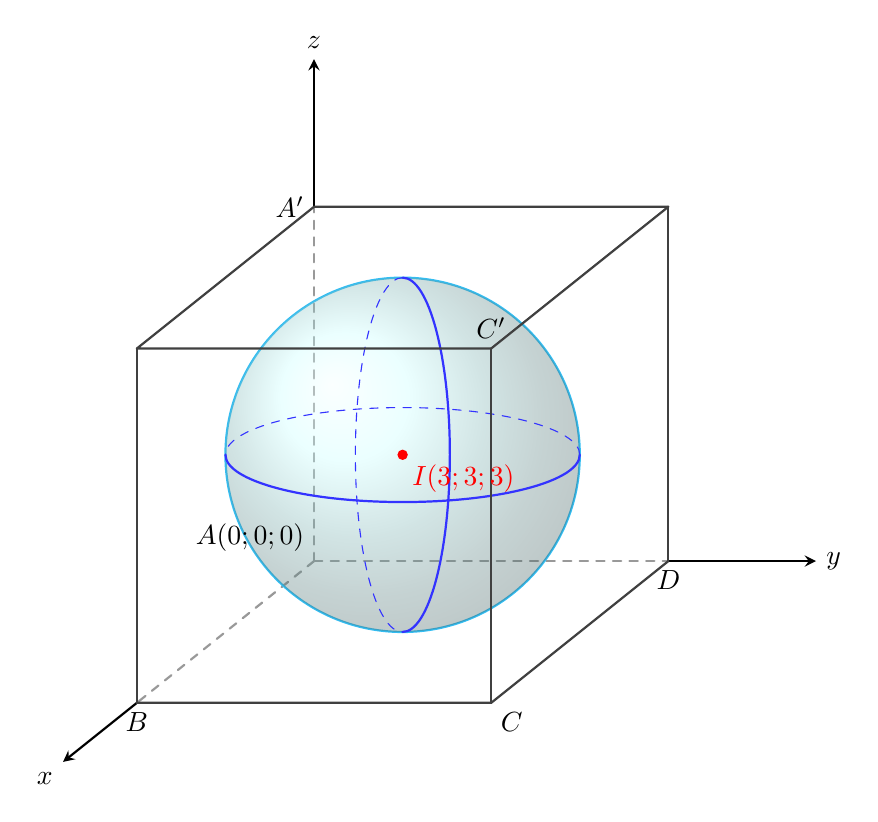
\begin{tikzpicture}[x={(-0.5cm,-0.4cm)}, y={(1.0cm,0cm)}, z={(0cm,1.0cm)}, scale=0.75, >=stealth, line join=round, line cap=round]
				% 1. Định nghĩa tọa độ các đỉnh của hình lập phương 6x6x6
				\coordinate (A) at (0,0,0);
				\coordinate (B) at (6,0,0);
				\coordinate (D) at (0,6,0);
				\coordinate (C) at (6,6,0);
				\coordinate (A') at (0,0,6);
				\coordinate (B') at (6,0,6);
				\coordinate (D') at (0,6,6);
				\coordinate (C') at (6,6,6);
				\coordinate (I) at (3,3,3); 
				
				% 2. Vẽ hệ trục phối hợp các cạnh khuất bên trong (Sửa lỗi nét đứt chuẩn xác)
				\draw[dashed, gray!80, thick] (A) -- (B);
				\draw[thick, ->] (B) -- (8.5,0,0) node[below left] {$x$};
				
				\draw[dashed, gray!80, thick] (A) -- (D);
				\draw[thick, ->] (D) -- (0,8.5,0) node[right] {$y$};
				
				\draw[dashed, gray!80, thick] (A) -- (A');
				\draw[thick, ->] (A') -- (0,0,8.5) node[above] {$z$};
				
				% 3. Vẽ khối cầu nội tiếp 
				\draw[cyan!80, thick] (I) circle [radius=3cm];
				\shade[ball color=cyan!30, opacity=0.35] (I) circle [radius=3cm];
				
				% Đường xích đạo mặt cầu
				\draw[blue!80, dashed, thin] (I) ++(3cm,0) arc (0:180:3cm and 0.8cm);
				\draw[blue!80, thick] (I) ++(-3cm,0) arc (180:360:3cm and 0.8cm);
				
				% Đường kinh tuyến mặt cầu
				\draw[blue!80, dashed, thin] (I) ++(0,3cm) arc (90:270:0.8cm and 3cm);
				\draw[blue!80, thick] (I) ++(0,-3cm) arc (-90:90:0.8cm and 3cm);
				
				% 4. Vẽ các cạnh nhìn thấy của hình lập phương
				\draw[thick, darkgray] (B) -- (C) -- (D);
				\draw[thick, darkgray] (A') -- (B') -- (C') -- (D') -- cycle;
				\draw[thick, darkgray] (B) -- (B') (C) -- (C') (D) -- (D');
				
				% 5. Đánh dấu điểm tâm I và dán nhãn các đỉnh
				\fill[red] (I) circle (2.5pt) node[below right, red] {$I(3;3;3)$};
				\node[above left] at (A) {$A(0;0;0)$};
				\node[below] at (B) {$B$};
				\node[below] at (D) {$D$};
				\node[left] at (A') {$A'$};
				\node[below right] at (C) {$C$};
				\node[above] at (C') {$C'$};
			\end{tikzpicture}
		\end{center}
		
		\begin{itemize}
			\item \textbf{Bước 1: Tính số phần tử của không gian mẫu $n(\Omega)$}\\
			Mỗi trục tọa độ gốc có $7$ giá trị nguyên chạy từ $0$ đến $6$. Số điểm nguyên thuộc khối lập phương là:
			\[ n(\Omega) = 7 \times 7 \times 7 = 343 \text{ (điểm)}.\]
			\item \textbf{Bước 2: Đếm số điểm thỏa mãn điều kiện bằng 2 cách khác nhau}\\
			Ta cần giải bài toán đếm số bộ số nguyên thỏa mãn: $X^2 + Y^2 + Z^2 \le 9$.
		\end{itemize}
		\textbf{CÁCH 1: TƯ DUY LÁT CẮT THEO TẦNG CAO (Chia nhỏ theo biến $Z$)}
		\\ Ta cho cao độ $Z$ chạy các giá trị nguyên từ $-3$ đến $3$. Lúc này bất phương trình đưa về dạng hình học phẳng: $X^2 + Y^2 \le 9 - Z^2$.
		\begin{itemize}
			\item \textbf{Tầng cao $Z = \pm 3$:} BPT trở thành $X^2 + Y^2 \le 0 \Rightarrow X=0, Y=0$.
			\\ $\rightarrow$ Mỗi tầng có đúng $1$ điểm. Tổng $2$ tầng: $1 \times 2 = 2$ điểm.
			\item \textbf{Tầng cao $Z = \pm 2$:} BPT trở thành $X^2 + Y^2 \le 5$.
			\begin{itemize}
				\item Nếu $X = 0 \Rightarrow Y^2 \le 5 \Rightarrow Y \in \{-2; -1; 0; 1; 2\}$ $\rightarrow$ có $5$ điểm.
				\item Nếu $X = \pm 1 \Rightarrow Y^2 \le 4 \Rightarrow Y \in \{-2; -1; 0; 1; 2\}$ $\rightarrow$ có $2 \times 5 = 10$ điểm.
				\item Nếu $X = \pm 2 \Rightarrow Y^2 \le 1 \Rightarrow Y \in \{-1; 0; 1\}$ $\rightarrow$ có $2 \times 3 = 6$ điểm.
			\end{itemize}
			$\rightarrow$ Tổng số điểm trên một tầng là $5 + 10 + 6 = 21$ điểm. Tổng $2$ tầng: $21 \times 2 = 42$ điểm.
			\item \textbf{Tầng cao $Z = \pm 1$:} BPT trở thành $X^2 + Y^2 \le 8$.
			\begin{itemize}
				\item Nếu $X = 0 \Rightarrow Y^2 \le 8 \Rightarrow Y \in \{-2; -1; 0; 1; 2\}$ $\rightarrow$ có $5$ điểm.
				\item Nếu $X = \pm 1 \Rightarrow Y^2 \le 7 \Rightarrow Y \in \{-2; -1; 0; 1; 2\}$ $\rightarrow$ có $2 \times 5 = 10$ điểm.
				\item Nếu $X = \pm 2 \Rightarrow Y^2 \le 4 \Rightarrow Y \in \{-2; -1; 0; 1; 2\}$ $\rightarrow$ có $2 \times 5 = 10$ điểm.
			\end{itemize}
			$\rightarrow$ Tổng số điểm trên một tầng là $5 + 10 + 10 = 25$ điểm. Tổng $2$ tầng: $25 \times 2 = 50$ điểm.
			\item \textbf{Tầng trung tâm $Z = 0$:} BPT trở thành $X^2 + Y^2 \le 9$.
			\begin{itemize}
				\item Nếu $X = 0 \Rightarrow Y^2 \le 9 \Rightarrow Y \in \{-3; -2; -1; 0; 1; 2; 3\}$ $\rightarrow$ có $7$ điểm.
				\item Nếu $X = \pm 1 \Rightarrow Y^2 \le 8 \Rightarrow Y \in \{-2; -1; 0; 1; 2\}$ $\rightarrow$ có $2 \times 5 = 10$ điểm.
				\item Nếu $X = \pm 2 \Rightarrow Y^2 \le 5 \Rightarrow Y \in \{-2; -1; 0; 1; 2\}$ $\rightarrow$ có $2 \times 5 = 10$ điểm.
				\item Nếu $X = \pm 3 \Rightarrow Y^2 \le 0 \Rightarrow Y = 0$ $\rightarrow$ có $2 \times 1 = 2$ điểm.
			\end{itemize}
			$\rightarrow$ Tổng số điểm trên tầng này là $7 + 10 + 10 + 2 = 29$ điểm.
		\end{itemize}
		$\Rightarrow$ Tổng số điểm thuận lợi thu được là: $n(E) = 2 + 42 + 50 + 29 = \mathbf{123}$ điểm.
		
		\vfill
		\textbf{CÁCH 2: TƯ DUY TỔ HỢP (Phân tích cấu trúc bộ bình phương)}
		\\ Vì $X, Y, Z$ nguyên nên bình phương của chúng chỉ có thể nhận các giá trị thuộc tập $\{0; 1; 4; 9\}$. Ta liệt kê tất cả các bộ số chưa tính thứ tự $\{X^2, Y^2, Z^2\}$ sao cho tổng của chúng không vượt quá $9$:
		\begin{enumerate}
			\item Bộ $\{0;0;0\}$ (Tổng bằng $0$): Có đúng $1$ điểm duy nhất là $(0;0;0)$.
			\item Bộ $\{1;0;0\}$ (Tổng bằng $1$): Số vị trí đặt số 1 là $\mathrm{C}_{3}^{1}=3$, chọn dấu ($\pm 1$) có $2$ cách $\rightarrow 3 \times 2 = 6$ điểm.
			\item Bộ $\{1;1;0\}$ (Tổng bằng $2$): Số vị trí đặt số 0 là $\mathrm{C}_{3}^{1}=3$, chọn dấu cho hai số 1 có $2^2=4$ cách $\rightarrow 3 \times 4 = 12$ điểm.
			\item Bộ $\{1;1;1\}$ (Tổng bằng $3$): Chọn dấu cho cả ba số 1 có $2^3 = 8$ cách $\rightarrow 8$ điểm.
			\item Bộ $\{4;0;0\}$ (Tổng bằng $4$): Số vị trí đặt số 4 là $\mathrm{C}_{3}^{1}=3$, chọn dấu ($\pm 2$) có $2$ cách $\rightarrow 3 \times 2 = 6$ điểm.
			\item Bộ $\{4;1;0\}$ (Tổng bằng $5$): Các số khác nhau đôi một nên có $3! = 6$ hoán vị vị trí, chọn dấu cho hai số khác không ($\pm 2, \pm 1$) có $2^2 = 4$ cách $\rightarrow 6 \times 4 = 24$ điểm.
			\item Bộ $\{4;1;1\}$ (Tổng bằng $6$): Số vị trí đặt số 4 là $\mathrm{C}_{3}^{1}=3$, chọn dấu cho ba số khác không có $2^3 = 8$ cách $\rightarrow 3 \times 8 = 24$ điểm.
			\item Bộ $\{4;4;0\}$ (Tổng bằng $8$): Số vị trí đặt số 0 là $\mathrm{C}_{3}^{1}=3$, chọn dấu cho hai số 4 có $2^2 = 4$ cách $\rightarrow 3 \times 4 = 12$ điểm.
			\item Bộ $\{4;4;1\}$ (Tổng bằng $9$): Số vị trí đặt số 1 là $\mathrm{C}_{3}^{1}=3$, chọn dấu cho ba số khác không có $2^3 = 8$ cách $\rightarrow 3 \times 8 = 24$ điểm.
			\item Bộ $\{9;0;0\}$ (Tổng bằng $9$): Số vị trí đặt số 9 là $\mathrm{C}_{3}^{1}=3$, chọn dấu ($\pm 3$) có $2$ cách $\rightarrow 3 \times 2 = 6$ điểm.
		\end{enumerate}
		$\Rightarrow$ Tổng số điểm thuận lợi tính theo cấu trúc là: $1 + 6 + 12 + 8 + 6 + 24 + 24 + 12 + 24 + 6 = \mathbf{123}$ điểm.
		\begin{itemize}
			\item \textbf{Bước 3: Tính toán giá trị xác suất cuối cùng}\\
			Xác suất hình học để chọn trúng điểm yêu cầu là
			\[ p = \dfrac{n(E)}{n(\Omega)} = \dfrac{123}{343}.\]
			Tính giá trị của biểu thức theo yêu cầu đề bài
			\[ 10000p = 10000 \times \dfrac{123}{343} \approx 3586.\]
		\end{itemize}
	}
\end{ex}